\chapter{Background}
\label{chap:background}

\section{Basics of Fully Homomorphic Encryption}
\gls{he} makes it possible to operate on data without knowing it.
One can distinguish three flavors of it, Partial-, Somewhat- and \gls{fhe}.

For \Gls{fhe}, there exist a few schemes in use today with existing implementations.
\begin{itemize}
  \item Brakerski/Fan-Vercauteren (BFV) scheme for integer arithmetic
        (\cite{2012-fv-original}, \cite{2012-brakerski}).
  \item Brakerski-Gentry-Vaikuntanathan (BGV) scheme for integer arithmetic \parencite{2012-bgv-original}.
  \item Cheon-Kim-Kim-Song (CKKS) scheme for real-number arithmetic \parencite{2017-ckks-original}.
  \item Ducas-Micciancio (FHEW) and Chillotti-Gama-Georgieva-Izabachene (TFHE) schemes for Boolean circuit evaluation
        \parencite{2019-tfhe-original}.
\end{itemize}

We will first introduce the BFV scheme (integer arithmetic) as it represents a fundamental building block behind CKKS.
Due to the inherent applications, this thesis will focus on the CKKS scheme to perform homomorphic operations
on (complex-valued) floating point numbers and vectors.

\subsection{Mathematical Foundation}
The following discussion of the homomorphic encryption schemes requires some mathematical background that
will (at least partially) be introduced here.

Let $\N$ denote the natural numbers without $0$, i.e. $\N = \{n \in \Z | n > 0\}$.
For a probability distribution $\chi$ over a set $R$, let sampling a value $x \in R$ from
the probability distribution be denoted by $x \leftarrow \chi$.
For $a \in \R$ a real number, denote rounding down (floor) $a$ by $\lfloor a \rfloor \in \Z$,
rounding up (ceil) by $\lceil a \rceil \in \Z$ and rounding to the nearest integer by
$\lfloor a \rceil \in \Z$.

\begin{definition}{Ring}{ring}
  A tuple $(R, +, \cdot)$ consisting of a set $R$, an addition operation $+$ and a multiplication operation $\cdot$
  is referred to as a ring, given that it satisfies the following \textit{ring axioms}:
  \begin{itemize}
    \item Addition is closed: $a + b \in R \quad\forall a, b \in R$.
    \item Addition is commutative: $a + b = b + a \quad\forall a, b \in R$.
    \item Addition is associative: $(a + b) + c = a + (b + c) \quad\forall a, b, c \in R$.
    \item There exists an element $0 \in R$ such that $a + 0 = a \quad\forall a \in R$.
    \item An additive inverse $-a$ of each element $a$ in $R$ exists, such that $a + (-a) = 0$.
    \item Multiplication is associative: $(a \cdot b) \cdot c = a \cdot (b \cdot c) \quad\forall a, b, c \in R$.
    \item Multiplication is closed: $a \cdot b \in R \quad\forall a, b \in R$.
    \item There exists an element $1 \in R$, referred to as the identity element, or multiplicative identity of $R$,
          such that $a \cdot 1 = a \quad\forall a \in R$.
    \item Multiplication $\cdot$ is distributive w.r.t. addition $+$, \\
          i.e. $a \cdot (b+c) = (a \cdot b) + (a \cdot c) \quad\forall a, b, c \in R$ from the left and \\
          i.e. $(b+c) \cdot a = (b \cdot a) + (c \cdot a) \quad\forall a, b, c \in R$ from the right.
  \end{itemize}
  Where the first 5 properties can be summarised as $(R, +)$ forming an Abelian group.
  If multiplication is additionally commutative, we refer to the ring as commutative:
  \begin{itemize}
    \item Multiplication is commutative: $a \cdot b = b \cdot a \quad\forall a, b \in R$.
  \end{itemize}
\end{definition}
Acting as a logical extension of a group, a ring can be considered the intermediary step towards a field
(which also defines subtraction and division).
An example of a ring would be the integers modulo $t$: $\Z / t \Z$, sometimes also denoted as $\Z_t$.

\begin{definition}{Quotient Group / Ring}{quotient-group}
  A quotient group $(G / N, +)$ (pronounced '$G$ mod $N$') over the original group $G$ and a normal subgroup $N$ of $G$
  with a standard element operation $+$ can be defined using the left cosets
  $$gN := \{gn \,|\, n \in N\} \subseteq G$$ of $N$ in $G$.
  The corresponding set $G / N$ is defined as
  $$G / N := \{g N \,|\, g \in G\}$$
  whereas the standard operation $+: G/N \times G/N \mapsto G/N$
  can be extended from the original group $G$ as follows:
  $$(gN) + (hN) := (gh)N$$
\end{definition}

\begin{definition}{Ring of Integers Modulo $t$: $\Z / t \Z$}{integers-modulo-t}
  Using equivalence classes $\overline{x}_t$ modulo $t$ referred to as congruence classes,
  define the commutative quotient ring of integers modulo $t$ as $(\Z / t \Z, +, \cdot)$ with
  two operations $+$ and $\cdot$ and
  $$\Z / t \Z = \{\overline{x}_t \,|\, x \in \Z, 0 \leq x < t\}$$
  where $t \Z \triangleleft \Z$ denotes the $t$\textsuperscript{th} coset\footnote{
    from the left and from the right, therefore $t \Z$ is called a normal subgroup of $\Z$
  } of the integers and
  $$\overline{x}_t = \{y \equiv x \mod t \,|\, y \in \Z\}$$
  is the set of all multiples of $t$ with remainder $x$.
  Note that many operations that resulting groups, rings or fields are commonly equipped with,
  such as addition or multiplication, propagate to an equivalent definition in the ring of integers modulo $t$
  by considering their result as a congruence class instead of it, which in turn is an element of $\Z / t \Z$.
\end{definition}

\begin{definition}{Polynomial Ring over $\Z$}{poly-ring}
  On the set of all complex-valued polynomials with integer coefficients (a function space)
  $$\Z[X] = \big\{p: \C \mapsto \C \,, p(X) = \sum_{k=0}^\infty a_k X^k, a_k \in \Z \;\forall k \geq 0\big\},$$
  we can define a commutative ring $(\Z[X], +, \cdot)$ equipped with the
  standard addition $+$ and multiplication $\cdot$ operations (as an extension over the field $\C$)
  of polynomials.
\end{definition}

% TODO: make p, q sequences instead of vectors
To further elaborate on the polynomial ring operations:
\begin{itemize}
  \item In their coefficient representations $(\vec{p})_i = p_0, p_1, p_2, ...$ (which are sequences) and $\vec{q} = \{q_0, q_1, q_2, ...\}$,
        an addition of two polynomials $p, q \in \Z[X]$ is equivalent to the addition of their coefficients
        \begin{align*}
          (p + q)(X) & = \sum_{k=0}^\infty p_k X^k + \sum_{k=0}^\infty q_k X^k = \sum_{k=0}^\infty (p_k + q_k) X^k \\
                     & = \langle (\vec{p} + \vec{q}), \{X^0, X^1, X^2, ...\}^T \rangle
        \end{align*}
        which indeed satisfies the additive \hyperref[def:ring]{ring axioms}
        due to the existing structure of the underlying field $\C$.
  \item The multiplication operation can be defined using a discrete convolution of the coefficient vectors
        $$r(X) = (p \cdot q)(X) = (\sum_{k=0}^\infty p_k X^k) \cdot (\sum_{l=0}^\infty q_l X^l)
          = \sum_{k=0}^\infty \sum_{l=0}^\infty p_k q_l X^{k+l}
          = \sum_{k=0}^\infty r_k X^k$$
        with the arising coefficients $\{r_k\}$ determined by the discrete convolution
        $$r_k = \sum_{l=0}^k p_l q_{k-l} \;\Leftrightarrow\; \vec{r} = \vec{p} * \vec{q}$$
        in this context also referred to as the \name{Cauchy}-product. Therefore,
        $$(p \cdot q)(X) = \langle (\vec{p} * \vec{q}), \{X^0, X^1, X^2, ...\}^T \rangle.$$
        Again, this generally applicable approach satisfies the multiplicative \hyperref[def:ring]{ring axioms}
        and even satisfies commutativity due to the existing structure of the underlying field $\C$
        and the symmetry of convolutions.
\end{itemize}

Where $\langle \cdot, \cdot \rangle$ denotes the dot (scalar) product between two vectors.

\begin{definition}{Irreducible Polynomials}{irreducible-polys}
  A polynomial is called irreducible \glstext{iff} it cannot be written as a product of other polynomials
  \textsl{while staying in the same coefficient space}.
\end{definition}

Polynomials with degree $\geq 1$ over the complex numbers can always be factorised using their roots
due to the fundamental theorem of algebra.

\subsection{Cyclotomic Polynomials}
Due to their interesting structure and efficient computability, in the following schemes,
polynomials modulo an irreducible form (\autoref{corollary:polys-mod}) are
chosen as representations of plaintexts and ciphertexts.
An important concept is that of cyclotomic ('circle-cutting') polynomials, which we will discuss
in a bit more detail here.

An important polynomial is $$p: \C \mapsto \C, \; p(x) = x^n - 1$$.
Its roots, found by solving $p(x) = 0$ for $x$, yielding $x^n = 1 \leftrightarrow x_k = \sqrt[n]{1}$
are referred to as the $n$\textsuperscript{th} roots of unity, of which there are multiple for each $n$.

\begin{lemma}{The $n$\textsuperscript{th} roots of unity}{nth-roots-of-unity}
  For some integer $n \in \N$, the $n$ complex roots $x_1, x_2, ..., x_n \in \C$ of unity
  can be found as $$x_k = e^{2\pi i \frac{k}{n}} \quad k \in \{1, 2, ..., n\}$$
  with $i$ the imaginary unit.
  Using \name{Euler}'s identity, their real and imaginary components can be explicitly found as
  $x_k = \cos(2\pi \frac{k}{n}) + i \sin(2\pi \frac{k}{n})$.

  An $n$\textsuperscript{th} root of unity $y$ is referred to as \textit{primitive}, \glstext{iff}
  there exists no $m < n$ for which that root $y$ is also an $m$\textsuperscript{th} root of unity, i.e. $y^m \neq 1$.
  An equivalent indicator is when $\gcd(m, n) = 1$.
\end{lemma}
Due to the fact that for any $k, l \in \Z$, their product $x_k \cdot x_l$ is also a root of unity, and
$x_{k+jn} = x_k \; \forall j \in \Z$, they clearly comprise a cyclic Abelian group over the complex numbers
$\C$ under multiplication with (for instance) the first root $x_1 = e^{2\pi i \frac{1}{n}}$ as its generator.

\begin{definition}{Cyclotomic Polynomial}{cyclotomic-poly}
  Given the $n$\textsuperscript{th} roots of unity $\{x_k\}$, we can define the $n$\textsuperscript{th}
  cyclotomic polynomial $\Phi_n \in \Z[X]$ as the product over all primitive roots of unity
  $$\Phi_n(x) = \prod_{\stackrel{k=1}{x_k \mathrm{primitive}}}^{n} (x - x_k)$$
  It is unique for each given $n \in \N$.
\end{definition}
The number of primitive roots of unity is given by $\varphi(n)$, denoting Euler's totient function which counts the
natural numbers $m$ less than $n$ who do not share a common divisor $\neq 1$, i.e. $\gcd(m, n) = 1$.
$\varphi(n)$ therefore also counts the number of primitive roots of unity for $n$,
consequently also yielding the degree of the $n$\textsuperscript{th} cyclotomic polynomial.

\begin{theorem}{$2^k$\textsuperscript{th} cyclotomic polynomial}{power-of-2-cyclo-poly}
  The $n$\textsuperscript{th} cyclotomic polynomial, where $n = 2^k$ ($k \in \N$) is a power of $2$,
  can be identified as
  $$\Phi_{n}(x) = x^{n/2} + 1\,.$$
  Its degree is $n/2$, consistent with $\varphi(2^k) = 2^{k-1} \; \forall k \in \N$.
\end{theorem}
Find a short but illustrative proof of \autoref{thm:power-of-2-cyclo-poly} in the \hyperref[chap:appendix]{Appendix}.

\begin{corollary}{Polynomials Modulo an Irreducible Form}{polys-mod}
  One can construct the interesting quotient ring
  $$\Z[X] / (X^N + 1)$$
  where $(X^N + 1)$ denotes the set of all polynomial multiples of the polynomial $p \in \Z[X], p(x) = x^n + 1$, so
  $$(X^N+1) = \{q: \C \mapsto \C,\; q(x) = r(x) \cdot (x^n+1) \;|\; r \in \Z[X]\}$$
  The elements of $R$ are $n$ polynomials with integer coefficients of degree $N-1$.
\end{corollary}

\begin{corollary}{Polynomial Ring modulo $q$}{polys-mod-q}
  Further modifying $R = \Z[X] / (X^N+1)$ to only take coefficients mod $q$, we obtain two equivalent definitions
  for the same ring:
  $$R/qR = (\Z/q\Z)[X] / (X^N+1) = \Z_q[X] / (X^N+1)$$
  which contains polynomials with integer coefficients modulo $q$ of degree $N-1$.
  Explicitly stated, the set can be written as:
  $$R/qR = \{p: \C \mapsto \C,\; p(x) = \sum_{k=0}^{N-1} a_k x^k \;|\; a_k \in \Z/q\Z\}$$
\end{corollary}

\begin{remark}{Irreducibility of Cyclotomic Polynomials}{cyclotomic-irreducibility}
  Cyclotomic polynomials are always irreducible.
\end{remark}
The proof for the above statement is quite cumbersome, but can be found in \cite{2002-serge-algebra}.

\subsection{HE using RSA}
In order to illustrate the basic idea behind \Gls{he}, without distancing ourselves too far
from the original goal of introducing basic \gls{he} operations used in practice, this short section aims to motivate
the definition of ring homomorphisms (cf. \autoref{def:ring-homomorphism}) behind a cryptographic background.

With unpadded RSA, some arithmetic can be performed on the ciphertext - % TODO: find RSA citation
looking at the encrypted ciphertext $\mathcal{E}(m_1) = (m_1)^r \mod n$
of the message $m_1$ and $m_2$ respectively, the following holds:
\begin{align*}
  \mathcal{E}(m_1) \cdot \mathcal{E}(m_2)
   & \equiv (m_1)^r (m_2)^r \mod n     \\
   & \equiv (m_1 m_2)^r \mod n         \\
   & \equiv \mathcal{E}(m_1 \cdot m_2)
\end{align*}

The encryption therefore partially fulfills the properties of a ring homomorphism,
which in general terms is defined as follows:

\begin{definition}{Ring Homomorphism}{ring-homomorphism}
  Given two \hyperref[def:ring]{rings} $(R, +, \cdot)$ and $(S, \oplus, \otimes)$, we call a mapping $\varphi: R \rightarrow S$
  a ring homomorphism when it satisfies the following conditions:
  $$\forall a, b \in R: \varphi(a + b) = \varphi(a) \oplus \varphi(b) \wedge \varphi(a \cdot b) =
    \varphi(a) \otimes \varphi(b)$$
\end{definition}

\subsection{Lattice Cryptography}

\subsection{Learning with Errors (LWE)}
\label{subsec:lwe}
Next, we would like to consider \Gls{lwe}, a computing problem that is believed to be sufficiently hard
to be used in cryptography and, most notably, is not yet solvable in linear time by a quantum algorithm
(c.f. \autoref{sec:post-quantum-sec}).
Its hardness assumptions were first formally proven by \citeauthor{2005-lwe-original},
for which he received the 2018 Gödel price.

\begin{definition}{LWE-Distribution $A_{\vec{s}, \chi_{error}}$}{lwe-dist}
  Given a prime $p \in \N$ and $n \in \N$, we choose some secret $\vec{s} \in (\Z / p \Z)^n$.
  In order to sample a value from the LWE distribution $A_{\vec{s}, \chi_{error}}$:
  \begin{itemize}
    \item Draw a random vector $a \in (\Z/p\Z)^n$ from the multivariate uniform distribution
          with its domain in the integers up to $p$.
    \item Given another probability distribution $\chi_{error}$ over the integers modulo $p$,
          sample a scalar 'error term' $\mu \in \Z / p \Z$ from it.
    \item Set $b = \vec{s} \cdot \vec{a} + \mu$, with $\cdot$ denoting the standard vector product.
    \item Output the pair $(\vec{a}, b) \in (\Z / p \Z)^n \times (\Z / p \Z)$.
  \end{itemize}
\end{definition}

The general approach useful to cryptography is to sample an element from the LWE-distribution and construct
two problems out of it, \textit{search}-LWE and \textit{decision}-LWE.

\begin{definition}{LWE-Problem - Search Version}{lwe-search-problem}
  Given $m$ independent samples $(\vec{a}_i, b_i)_{0 < i \leq m}$ from $A_{\vec{s}, \chi_{error}}$, find the secret $\vec{s}$.
\end{definition}
\begin{definition}{LWE-Problem - Decision Version}{lwe-decision-problem}
  Given $m$ samples $(\vec{a}_i, b_i)_{0 < i \leq m}$, distinguish (with non-negligible advantage)
  whether they were drawn from $A_{\vec{s}, \chi_{error}}$ or from the uniform distribution
  $u$ over $(\Z / p \Z)^n \times (\Z / p \Z)$.
\end{definition}

In their above definitions, \citeauthor{2005-lwe-original} showed that the two problems are equivalent.

To illustrate the connection of these problems to lattices, we
take a closer look at them before considering further details of LWE.
Most notably, lattice problems are conjectured to be secure against quantum computers \parencite{2018-lattice-problems}.

\newcommand{\lat}{\mathcal{L}}
\begin{definition}{Lattice}{lattice}
  A lattice $(\lat, +, \cdot)$ is a vector field over the integers $(\Z, +, \cdot)$, defined using a set of $n$
  basis vectors $\vec{b_1}, \vec{b_2}, ..., \vec{b_n} \in \R^n$, that can be introduced as a set
  $$\lat = \bigg\{\sum_{i=1}^m c_i \vec{b}_i \,|\, c \in \Z\bigg\} \subseteq \R^n$$
  equipped with at least vector addition $+: \lat \times \lat \mapsto \lat$
  and scalar multiplication $\cdot: \Z \times \lat \mapsto \lat$.
  As an extension of $\R^n$, the Euclidean norm $||\cdot||$ is also defined and
  the standard Euclidean metric $d: \lat \times \lat \mapsto \R$, yielding a metric space $(\lat, d)$,
  can be obtained by the norm of a vector difference, denoted $||(\cdot) - (\cdot)||$.
\end{definition}

Its \textit{minimum distance} $\lambda_{min}$ is defined as the smallest Euclidean distance
between two points $\vec{p_1}$ and $\vec{p_2} \in \lat$
$$\lambda_{min} = \min_{\vec{p_1}, \vec{p_2} \in \lat} d(\vec{p_1}, \vec{p_2}) =
  \min_{\vec{p_1}, \vec{p_2} \in \lat} ||\vec{p_1} - \vec{p_2}|| \,,$$
which can be equivalently thought of as the minimal length of any non-zero vector in the lattice $\lat$,
because of $\vec{0}$ always being an element of the lattice which can be chosen as $\vec{p_1}$
and the translational symmetry between fundamental lattice volumes (or regions).

\begin{definition}{Shortest Vector Problem (SVP)}{svp}
  Given a lattice $\lat$ constructed from $n$ basis vectors,
  find the shortest non-zero lattice vector $\vec{x} \in \lat \backslash \{\vec{0}\}$,
  i.e. find $\vec{x}$ such that $||\vec{x}|| = \lambda_{min}$ \parencite{2016-decade-of-lattice}.
\end{definition}

\begin{definition}{Decisional Approximate SVP (GapSVP)}{gap-svp}
  Given a lattice $\lat$ and some pre-defined function $\gamma: \N \mapsto \R$ depending
  on the lattice dimension $n$ (constant for a given $\lat$) with $\gamma(n) \geq 1$,
  the decisional approximate shortest vector problem is distinguishing
  between $\lambda_{min} \leq 1$ and $\lambda_{min} > \gamma(n)$.
  For other cases, it is up to the algorithm what to return.
\end{definition}

\begin{definition}{Short Integer Solution (SIS) Problem}{sis}
  For $m$ given vectors $(\vec{a}_i)_{0 < i \leq m} \in (\Z / q\Z)^n$ that comprise the columns of a matrix
  $A \in (\Z / q\Z)^{n \times n}$ and an upper bound $\beta$, find
  a solution vector $\vec{z} \in \Z^n \backslash \{\vec{0}\}$ such that
  $$A \vec{z} = \vec{0} \quad \mathrm{with} \quad ||\vec{z}|| \leq \beta\,.$$
\end{definition}

Note that without the last requirement, the SIS problem can be easily solved through Gaussian elimination or
similar algorithms, however they rarely yield a short (or \textit{the} shortest) solution.
It can be shown that solving SIS is at least as hard as solving GapSVP with appropriate parameters
\parencite{1996-hard-lattice-problems}.

Using the above problems, multiple cryptographic primitives can be constructed
due to the proven hardness that also propagates to quantum computers.
Examples include collision resistant hash functions, signatures, pseudorandom functions
or even Regev's public-key cryptosystem \parencite{2016-decade-of-lattice}.

\usetikzlibrary{calc}
\begin{figure}
  \centering
  \begin{tikzpicture}
    \coordinate (Origin)   at (0,0);
    \coordinate (XAxisMin) at (-3,0);
    \coordinate (XAxisMax) at (5,0);
    \coordinate (YAxisMin) at (0,-2);
    \coordinate (YAxisMax) at (0,5);
    \draw [thin, gray,-latex] (XAxisMin) -- (XAxisMax);
    \draw [thin, gray,-latex] (YAxisMin) -- (YAxisMax);

    \clip (-3,-2) rectangle (6.5cm, 6.5cm);
    \pgftransformcm{1}{0.3}{0.7}{1}{\pgfpoint{0cm}{0cm}}
    \coordinate (Bone) at (0,2);
    \coordinate (Btwo) at (2,-2);
    \draw[style=help lines,dashed] (-14,-14) grid[step=2cm] (14,14);
    \foreach \x in {-7,-6,...,7}{
        \foreach \y in {-7,-6,...,7}{
            \node[draw,circle,inner sep=2pt,fill] at (2*\x,2*\y) {};
          }
      }
    \draw [ultra thick,-latex,themecolor] (Origin)
    -- (Bone) node [above left] {$\vec{b}_1$};
    \draw [ultra thick,-latex,themecolor] (Origin)
    -- (Btwo) node [below right] {$\vec{b}_2$};
  \end{tikzpicture}
  \caption{Illustration of a standard lattice $\lat$ over the integers $\Z$
    with two basis vectors $\vec{b}_1$ and $\vec{b}_2$, c.f. \autoref{def:lattice}.
    The shortest vector problem in this case is solved by $\vec{x} = 0 \vec{b}_1 \pm 1 \vec{b}_2$.}
  \label{fig:lattice}
\end{figure}

\begin{theorem}{Hardness of LWE}{lwe-hardness}
  If there exists an efficient algorithm that solves either search-LWE or decision-LWE then
  there exists an efficient quantum algorithm that approximates the decision
  version of the shortest vector problem (GapSVP) in the worst case \parencite{2010-lwe-survey}.
\end{theorem}

He also provided a construction of a public-key cryptosystem based on them, i.e. an asymmetric cryptographic
system for at least two parties that includes a public and corresponding private key.

Public-key cryptosystems are fundamentally different from symmetric systems, which only
require one single key for encryption and decryption at the same time, known by all involved parties.
Often times, public-key schemes (rather slow) are used to exchange keys for subsequent symmetric encryption
(rather fast) of large plaintexts, for instance in the \gls{tls} protocol \parencite{rfc8446}.

\subsection{Ring-LWE}
\Gls{rlwe}
\cite{2010-rlwe-original}
% TODO: how to get from LWE to RLWE

Similar to \autoref{def:lwe-dist}, the Ring-LWE distribution can be derived as follows:

\begin{corollary}{RLWE-Distribution $B_{\vec{s}, \chi_{error}}$}{rlwe-dist}
  Given a quotient \hyperref[def:ring]{ring} $(R/qR, +, \cdot)$, we choose some secret $s \in R/qR$.
  In order to sample a value from the RLWE distribution $B_{s, \chi_{error}}$:
  \begin{itemize}
    \item Uniformly randomly draw an element $a \in R/qR$
    \item Given another probability distribution $\chi_{error}$ over the ring elements,
          sample an 'error term' $\mu \in R/qR$ from it.
    \item Set $b = s \cdot a + \mu$, with $\cdot$ denoting the ring multiplication operation.
    \item Output the pair $(a, b) \in R/qR \times R/qR$.
  \end{itemize}
\end{corollary}

In the exact same manner as \hyperref[subsec:lwe]{above}, the search and decision problems
can be constructed.

\begin{corollary}{RLWE-Search Problem}{search-rlwe}
  Given $m$ independent samples $(a_i, b_i)_{0 < i \leq m}$ from $B_{s, \chi_{error}}$, find the secret $s$.
\end{corollary}
\begin{corollary}{RLWE-Decision Problem}{decision-rlwe}
  Given $m$ samples $(a_i, b_i)_{0 < i \leq m}$, distinguish (with non-negligible advantage)
  whether they were drawn from $B_{s, \chi_{error}}$ or from the uniform distribution
  $u$ over $R/qR \times R/qR$.
\end{corollary}

\subsection{Gentry's FHE-Scheme and BGV}
\cite{2009-gentry-fhe-original}
% TODO: historical introduction

\pagebreak
\subsection{The BFV scheme}
\cite{2012-fv-original}
\cite{2012-brakerski}
BFV is based on BGV and they are very similar in the core ideas,
one can even convert a BFV ciphertext to an equivalent BGV ciphertext \parencite{2021-he-revisiting}.

In this section, we will focus on a slightly altered implementation introduced in \cite{2014-fv-comparison}.

\newcommand{\cryptop}[1]{\text{\textcolor{darkpurple}{#1}}}
\begin{definition}{The BFV-Scheme}{bfv-scheme}
  Let $R = \Z[X] / \Phi_d(X)$ be a ring with $\Phi_d(X)$ the $d$\textsuperscript{th} \hyperref[def:cyclotomic-poly]{cyclotomic polynomial}
  ($\rightarrow d \in \N$) for ciphertexts $c \in R \times R$.
  Introduce $R / qR$ the associated quotient ring of the $q$\textsuperscript{th} coset of $R$ with the modulus $q \in \N$.
  Further let $t \in \N$ denote the message modulus with $1<t<q$
  for plain messages $m \in R/tR$ and define $\delta = \lfloor \frac{q}{t} \rfloor$,
  $\delta^{-1} = \frac{t}{q}$.

  Introduce two bounded discrete probability distributions $\chi_{key}$ and $\chi_{error}$ over $R/qR$,
  one which is only used once for key generation and another (usually Gaussian-like) error distribution
  for the \hyperref[def:lwe-search-problem]{LWE-problem}.

  For a polynomial $a \in R/qR$, consider the decomposition $a = \sum_{i=0}^{l-1} a_i w^i$ into base $w \in \N$
  obtained by $\cryptop{WordDecomp}: R \mapsto R^l, \cryptop{WordDecomp}(a) = ([a_i]_w)_{i=0}^{l-1}$. \\
  Further let $\cryptop{PowersOf}: R \mapsto R^l$ be defined as $\cryptop{PowersOf}(a) = ([a w^i]_q)_{i=0}^{l-1}$.

  Let the parameters $\mathbb{P} = (d, q, t, \chi_{key}, \chi_{error}, w)$ and $l = \lfloor \log_w(q) \rfloor + 1$.
  \vspace{0.4cm}

  \begin{tblr}{Q[l,h]Q[l,h,\textwidth - 3.5cm]}
    \cryptop{ParamGen}$(\lambda)$ & {
        Choose parameters as defined above, given the
        security parameter $\lambda$, such that $1 < t < q$, $w \geq 2$,
        initialize distributions $\chi_{key}$ and $\chi_{error}$
        $\quad\rightarrow \mathbb{P}$} \\
    \cryptop{KeyGen}$(\mathbb{P})$ & {
        Generate the secret key $s \leftarrow \chi_{key}$, sample $\vec{\mu} \in (R/qR)^l$
        from $\chi_{error}$ and choose some $\vec{a} \in (R/qR)^l$ uniformly
        at random, compute the relinearization key
        $\vec{\gamma} = (\cryptop{PowersOf}(s^2) - (\vec{\mu} + \vec{a} \cdot s), \vec{a})$
        and finally output the public key for uniformly random
        $a \in (R/qR)$ and $\mu \leftarrow \chi_{error}$ with $b =-(a \cdot s + \mu)$
        as $\vec{p} = (b, a)$.
        $\quad\rightarrow \vec{p}, s, \vec{\gamma}$} \\
    \cryptop{Encrypt}$(\vec{p}, m)$ & {
        Let $(b,a) = \vec{p}$, $u \leftarrow \chi_{key}$, $\mu_1, \mu_2 \leftarrow \chi_{error}$,
        then the ciphertext is $\vec{c} = (\delta m + bu + \mu_1, au + \mu_2)$
        $\quad\rightarrow \vec{c}$} \\
    \cryptop{Add}$(\vec{c}_1, \vec{c}_2)$ & {
        Let $(c_0^1, c_1^1) = \vec{c}_1$ and $(c_0^2, c_1^2) = \vec{c}_2$
        then $\vec{c}_3 = (c_0^1 + c_0^2, c_1^1 + c_1^2)$
        $\quad\rightarrow \vec{c}_3$} \\
    \cryptop{Mult}$(\vec{c}_1, \vec{c}_2)$ & {
        Output $\overline{\vec{c}} = (
          \lfloor \delta^{-1} c_0^1 c_0^2 \rceil,
          \lfloor \delta^{-1}(c_0^1 c_1^2 + c_1^1 c_0^2) \rceil,
          \lfloor \delta^{-1} c_1^1 c_1^2 \rceil
          )$
        $\quad\rightarrow \overline{\vec{c}}$} \\
    \cryptop{ReLin}$(\overline{\vec{c}}, \vec{\gamma})$ & {
        Using the relin key $\vec{\gamma} = (\vec{b}, \vec{a})$,
        relinearize from $\overline{\vec{c}} = (c_0, c_1, c_2)$ as
        $\vec{c} = (c_0 + \cryptop{WordDecomp}(c_2) \cdot \vec{b}, c_1 + \cryptop{WordDecomp}(c_2) \cdot \vec{a})$
        $\quad\rightarrow \vec{c}$} \\
    \cryptop{Decrypt}$(s, \vec{c})$ & {
        And finally, decrypt $\vec{c} = (c_0, c_1)$ as
        $m = \lfloor \delta^{-1} [c_0 + c_1 s]_q \rceil \in R/tR$
        $\quad\rightarrow m$} \\
  \end{tblr}

  \parencite{2012-fv-original, 2012-brakerski}
\end{definition}

To summarise the parameters and variables, a brief overview of all used symbols is
provided in \autoref{tab:bfv-symbols}.
\begin{table}[H]
  \centering
  \caption{Summary of the parameters and symbols in BFV.}
  \begin{tblr}{rll}
    \hline
    \textbf{Symbol} & \textbf{Space} & \textbf{Explanation} \\
    \hline
    $\lambda$ & $\in \R$ & Security parameter \\
    $d$ & $\in \N$ & Index of the cyclotomic polynomial over $R$ \\
    $q$ & $\in \N$ & Modulus of the ciphertext space $R/qR$ \\
    $t$ & $\in \N$ & Modulus of the plaintext message space $R/tR$ \\
    $\delta$ & $\in \N$ & Ratio between ciphertext and plaintext modulus \\
    $\delta^{-1}$ & $\in \R$ & Inversion coefficient of the effect of $\delta$ \\
    $w$ & $\in \N$ & Word size used as basis, e.g. $w = 2$ for bits \\
    $l$ & $\in \N$ & Number of words of size $w$ required to encode $q$ \\
    $s$ & $\in R$ & Secret Key \\
    $\vec{p}$ & $\in R/qR \times R/qR$ & Public Key $(b, a)$ \\
    $\vec{\gamma}$ & $\in (R/qR)^l \times (R/qR)^l$ & Relinearization Key \\
    $m$ & $\in R/tR$ & Plaintext Message\\
    $\vec{c}$ & $\in R \times R$ & Ciphertext \\
    $\overline{\vec{c}}$ & $\in R \times R \times R$ & Slightly larger ciphertext resulting from multiplication \\
  \end{tblr}
  \label{tab:bfv-symbols}
\end{table}


\tikzstyle{cleartext} = [rectangle, rounded corners,minimum width=3cm, minimum height=1cm, text centered, draw=black, fill=orange!30]
\tikzstyle{plaintext} = [rectangle, rounded corners,minimum width=3cm, minimum height=1cm, text centered, draw=black, fill=purple!30]
\tikzstyle{ciphertext} = [rectangle, rounded corners,minimum width=3cm, minimum height=1cm, text centered, draw=black, fill=themecolor!30]
\tikzstyle{arrow} = [thick,->,>=stealth]

\begin{figure}[H]
  \centering
  \begin{tikzpicture}
    \node[cleartext, align = center] (m) at (0,0) {message \\ $m$};
    \node[plaintext, align = center] (p) at (6,0) {plaintext \\ $p(X)$};
    \node[ciphertext, align = center] (c) at (12,0) {ciphertext \\ $c = (c_0(X), c_1(X))$};

    \node[cleartext, align = center] (m2) at (0,-2.5) {message \\ $\tilde{m}=f(m)$};
    \node[plaintext, align = center] (p2) at (6,-2.5) {plaintext \\ $\tilde{p}(X) = f(p(X))$};
    \node[ciphertext, align = center] (c2) at (12,-2.5) {ciphertext \\ $\tilde{c} = f(c)$};

    \draw (m.north) node[above]{$\C^{N/2}$};
    \draw (m2.south) node[below]{$\C^{N/2}$};
    \draw (p.north) node[above]{$\Z[X]/(X^N + 1)$};
    \draw (p2.south) node[below]{$\Z[X]/(X^N + 1)$};
    \draw (c.north) node[above]{$(\Z_q[X]/(X^N + 1))^2$};
    \draw (c2.south) node[below]{$(\Z_q[X]/(X^N + 1))^2$};

    \draw [arrow] (m) -- node[anchor=south] {encoding} (p) ;
    \draw [arrow] (p) -- node[anchor=south] {encryption} (c);
    \draw [arrow] (c) -- node[anchor=east] {computing $f$} (c2);
    \draw [arrow] (c2) -- node[anchor=south] {decryption} (p2);
    \draw [arrow] (p2) -- node[anchor=south] {decoding} (m2);
  \end{tikzpicture}
  \caption{Overview of BFV, adapted from \cite{2020-cryptotree}.}
  \label{fig:bfv-overview}
\end{figure}

\begin{theorem}{BFV encryption is homomorphic with respect to addition}{bfv-enc-is-homomorphic}
  \cryptop{BFV.Encrypt} should encrypt in such a way that the addition algebra can be retained
  even in the transformed space, showing that we can indeed refer to it as homomorphic encryption.
\end{theorem}

\subsection{The CKKS scheme}
The CKKS scheme allows us to perform approximate arithmetic on floating point numbers.
Essentially, the idea is to extend BFV which allows us to operate on vectors $\vec{y} \in \Z_t^n$,
by an embedding approach that allows us to encode a (complex) floating point number vector $\vec{x} \in \R^n (\C^n)$
as an integer vector. A na\"ive approach would be to use a fixed-point embedding:
\newcommand{\embed}{\mathrm{embed}}
$$\embed(\vec{x}) = \vec{x} \cdot F$$
with $F \in \Z$. In decimal form, for instance with $F = 1000$, we could effectively encode
three decimal places of the original vector $\vec{x}$.
% ... TODO: scale explodes, confer Roman's PETS lecture -> motivation for CKKS.

\tikzstyle{cleartext} = [rectangle, rounded corners,minimum width=3cm, minimum height=1cm, text centered, draw=black, fill=orange!30]
\tikzstyle{plaintext} = [rectangle, rounded corners,minimum width=3cm, minimum height=1cm, text centered, draw=black, fill=purple!30]
\tikzstyle{ciphertext} = [rectangle, rounded corners,minimum width=3cm, minimum height=1cm, text centered, draw=black, fill=themecolor!30]
\tikzstyle{arrow} = [thick,->,>=stealth]

\begin{figure}[H]
  \centering
  \begin{tikzpicture}
    \node[cleartext, align = center] (m) at (0,0) {message \\ $m$};
    \node[plaintext, align = center] (p) at (6,0) {plaintext \\ $p(X)$};
    \node[ciphertext, align = center] (c) at (12,0) {ciphertext \\ $c = (c_0(X), c_1(X))$};

    \node[cleartext, align = center] (m2) at (0,-2.5) {message \\ $\tilde{m}=f(m)$};
    \node[plaintext, align = center] (p2) at (6,-2.5) {plaintext \\ $\tilde{p}(X) = f(p(X))$};
    \node[ciphertext, align = center] (c2) at (12,-2.5) {ciphertext \\ $\tilde{c} = f(c)$};

    \draw (m.north) node[above]{$\C^{N/2}$};
    \draw (m2.south) node[below]{$\C^{N/2}$};
    \draw (p.north) node[above]{$\Z[X]/(X^N + 1)$};
    \draw (p2.south) node[below]{$\Z[X]/(X^N + 1)$};
    \draw (c.north) node[above]{$(\Z_q[X]/(X^N + 1))^2$};
    \draw (c2.south) node[below]{$(\Z_q[X]/(X^N + 1))^2$};

    \draw [arrow] (m) -- node[anchor=south] {encoding} (p) ;
    \draw [arrow] (p) -- node[anchor=south] {encryption} (c);
    \draw [arrow] (c) -- node[anchor=east] {computing $f$} (c2);
    \draw [arrow] (c2) -- node[anchor=south] {decryption} (p2);
    \draw [arrow] (p2) -- node[anchor=south] {decoding} (m2);
  \end{tikzpicture}
  \caption{Overview of CKKS, adapted from \cite{2020-cryptotree}.}
  \label{fig:ckks-overview}
\end{figure}

% \subsubsection{Packing}
% FFT in CKKS!
% (Polynom -> Vektor) mit einer FFT
% (Vektor -> Polynom) mit einer IFFT

\begin{theorem}{CKKS encryption is homomorphic with respect to addition}{ckks-enc-is-homomorphic}
  \cryptop{CKKS.Encrypt} should encrypt in such a way that the addition algebra can be retained
  even in the transformed space, showing that we can indeed refer to it as homomorphic encryption.
\end{theorem}

\textit{Microsoft SEAL} implements the scheme, enabled using \cpp{seal::scheme_type::ckks}.

\pagebreak
\section{Machine Learning}
Undoubtedly one of the most prevalent concepts in todays computing world, \gls{ml} has shaped
how computers think and how we interact with them significantly.
As Shafi \name{Goldwasser} puts it, 'Machine Learning is somewhere in the intersection of Artificial Intelligence,
Statistics and Theoretical Computer Science' \parencite{goldwasserTalk2018}.

Within the scope of this thesis, the basics of neural networks and associated learning methods shall be covered,
limited to the category of supervised learning problems (as opposed to unsupervised learning problems).
Supervised learning refers to the machine \textit{training} an algorithm to match some input data (features)
with corresponding output data (targets), often related to pattern recognition.
The trained algorithm can then be utilised to match fresh input data with a prediction of the targets.

A popular subset of applications to \gls{ml} are classification problems, predominantly image classification,
which was not as easily possible before without a human eye due to the lack of computing power.
Classification problems can be formulated quickly, the goal is to computationally categorize input data
(for instance, images) into a predefined set of classes (for instance, cats and dogs).
The primary concept behind \acrlong{ml} is not at all new, linear regression
was already employed by \name{Gauß} and \name{Legendre} in the early 19\textsuperscript{th} century;
the term 'Neural Network' was first used by \name{McCulloch} and \name{Pitts} in 1943.
Much media attention was earned in the 2000-2010 decade when larger image classification problems
became feasible with the increasing computational power of modern computers,
up until the advent of Deep Learning \parencite{bishop-pattern-recognition-and-ml}.

\subsection{Linear Regression}
Given an input vector $\vec{x} \in \R^n$, the goal of linear regression is to predict the value of a target $t \in \R$,
according to some model $M$.

\subsection{Gradient Descent}
\subsection{Multi-Layered Neural Networks}

\begin{theorem}{Universal Approximation}
  If the neural network has at least one hidden layer, proper nonlinear activation functions and enough
  data and hidden units, it can approximate any continuous function $y(x, w): \R^n \mapsto \R$
  arbitrarily well on a compact domain
  \parencite{1989-HornikMultilayerFN}.
\end{theorem}

Matrix -> Activation Function
\begin{itemize}
  \item Matrix Multiplication (Dense Layer)
  \item Convolutional Layer
  \item Sigmoid Activation
  \item Max Pooling
\end{itemize}

\subsection{The Backpropagation Algorithm}

\section{Post-Quantum Security}
\label{sec:post-quantum-sec}
\subsection{Shor's Algorithm}

\begin{figure}[H]
  \centering
  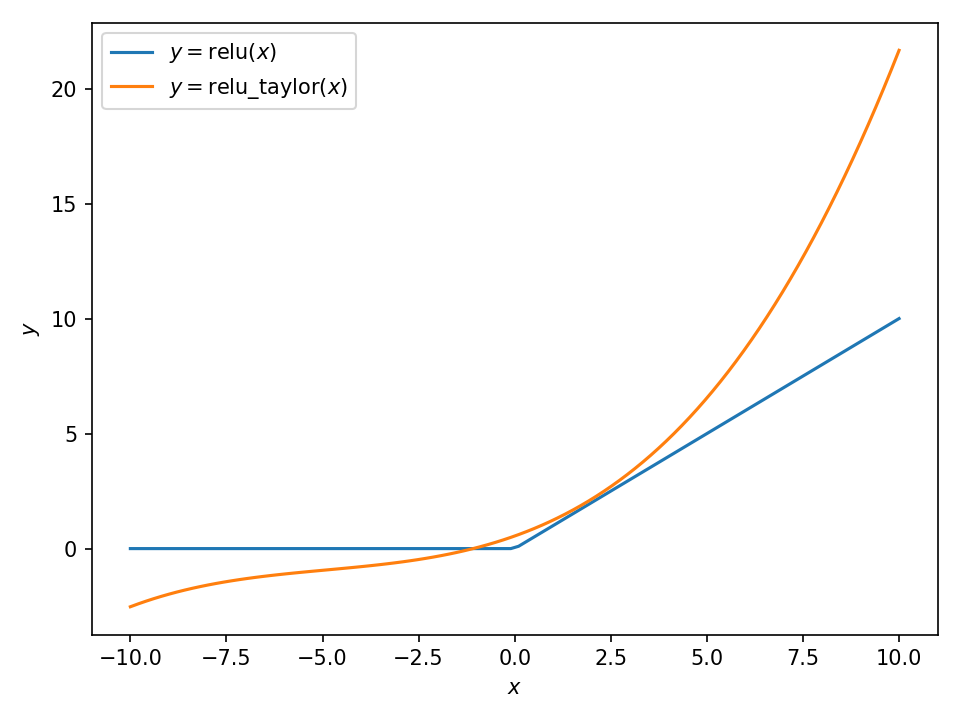
\includegraphics[width=0.8\linewidth]{figures/taylor-relu.png}
  \caption{Comparison of the Relu activation function vs. its Taylor expansion}
\end{figure}
